\documentclass[letterpaper]{article}
\usepackage{underscore}
\usepackage[left=2.0cm, right=2.0cm, top=2.0cm]{geometry}
\usepackage[utf8]{inputenc}
\usepackage{graphicx}
\usepackage{graphics}
\usepackage[spanish]{babel}
\usepackage{lipsum}
\usepackage{float}
\usepackage{subfigure}
\usepackage{biblatex}
\usepackage{csquotes}
\usepackage{color}

\title{2\_6\_Construir\_un\_amplificación\_con\\\_conexion\_Darlington}
\author{Alcantar Diaz Joel Alejandro\\ \& \\Ledesma Hernández Miguel Ángel}
\date{09/11/2019}

\begin{document}

\maketitle
\vspace{2 cm}
\begin{large}
    \begin{center}
        
\includegraphics[width=7cm]{IMG/UPZMGlog.png}\\
        Universidad Politécnica de la Zona Metropolitana de Guadalajara.\\
        Ingeniería Mecatrónica.\\
        $4^{to}$ A
    \end{center}
\end{large}
\newpage
\section{Objetivo:}
\begin{large}
    Construir circuitos de amplificación con transistores darlington.
\end{large}
\section{Materiales:}
\begin{large}
    \begin{table}[htbp]
        \centering
        \begin{tabular}{|l|l|}
            \hline
            Materiales            & Equipo \\ \hline
            Transistor TIP112     & Fuente de alimentación \\ \hline
            Protoboard            & Contactor \\ \hline
            LED                   & \\ \hline
            LDR                   & \\ \hline
            Resistencias varias   & \\ \hline
            Cable para protoboard & \\ \hline
            Potenciómetro         & \\ \hline
            Relay                 & \\ \hline
        \end{tabular}
    \end{table}
\end{large}
\section{Procedimiento: Circuito detector de luz.}
\begin{large}
    \begin{enumerate}
        \item Conectar una resistencia de 100$\Omega$ a un potenciómetro de 10K$\Omega$ y el potenciómetro a el LDR o foto-resistencia como se muestra en la figura 1.
        \begin{figure}[htbp]
            \centering
            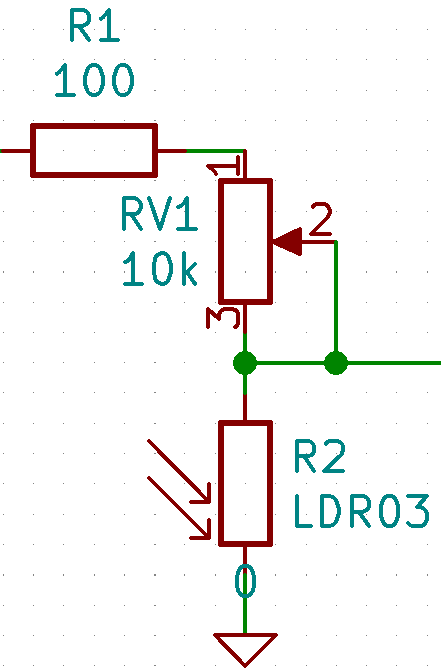
\includegraphics[scale=0.4]{IMG/CIRLuz2.png}
            \caption{Circuito de resistivo.}
            \label{fig:cir1}
        \end{figure}
        \item Se conecta de entre el potenciómetro a la base del Darlington y colector a la bobina del relay.
        \item Conectar el otro extremo de la bobina del relay a tierra como en la figura 2
        \newpage
        \begin{figure}[htbp]
            \centering
            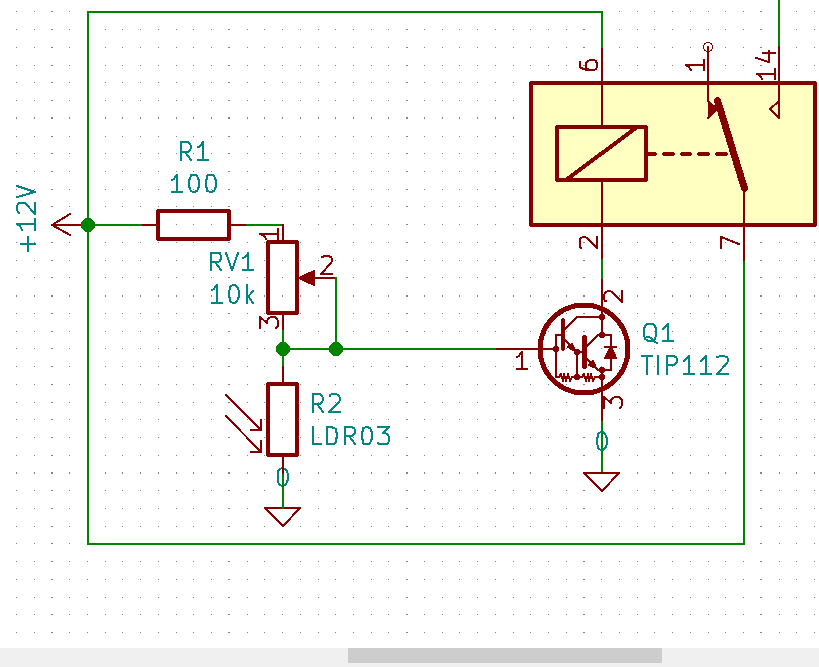
\includegraphics[scale=0.4]{IMG/criluz4.png}
            \caption{Circuito con relay}
            \label{fig:relcir}
        \end{figure}
        \item Se agrega el circuito del LED conectado a comúnmente abierto en el relay quedando el circuito como el de la figura 3
        \begin{figure}[htbp]
            \centering
            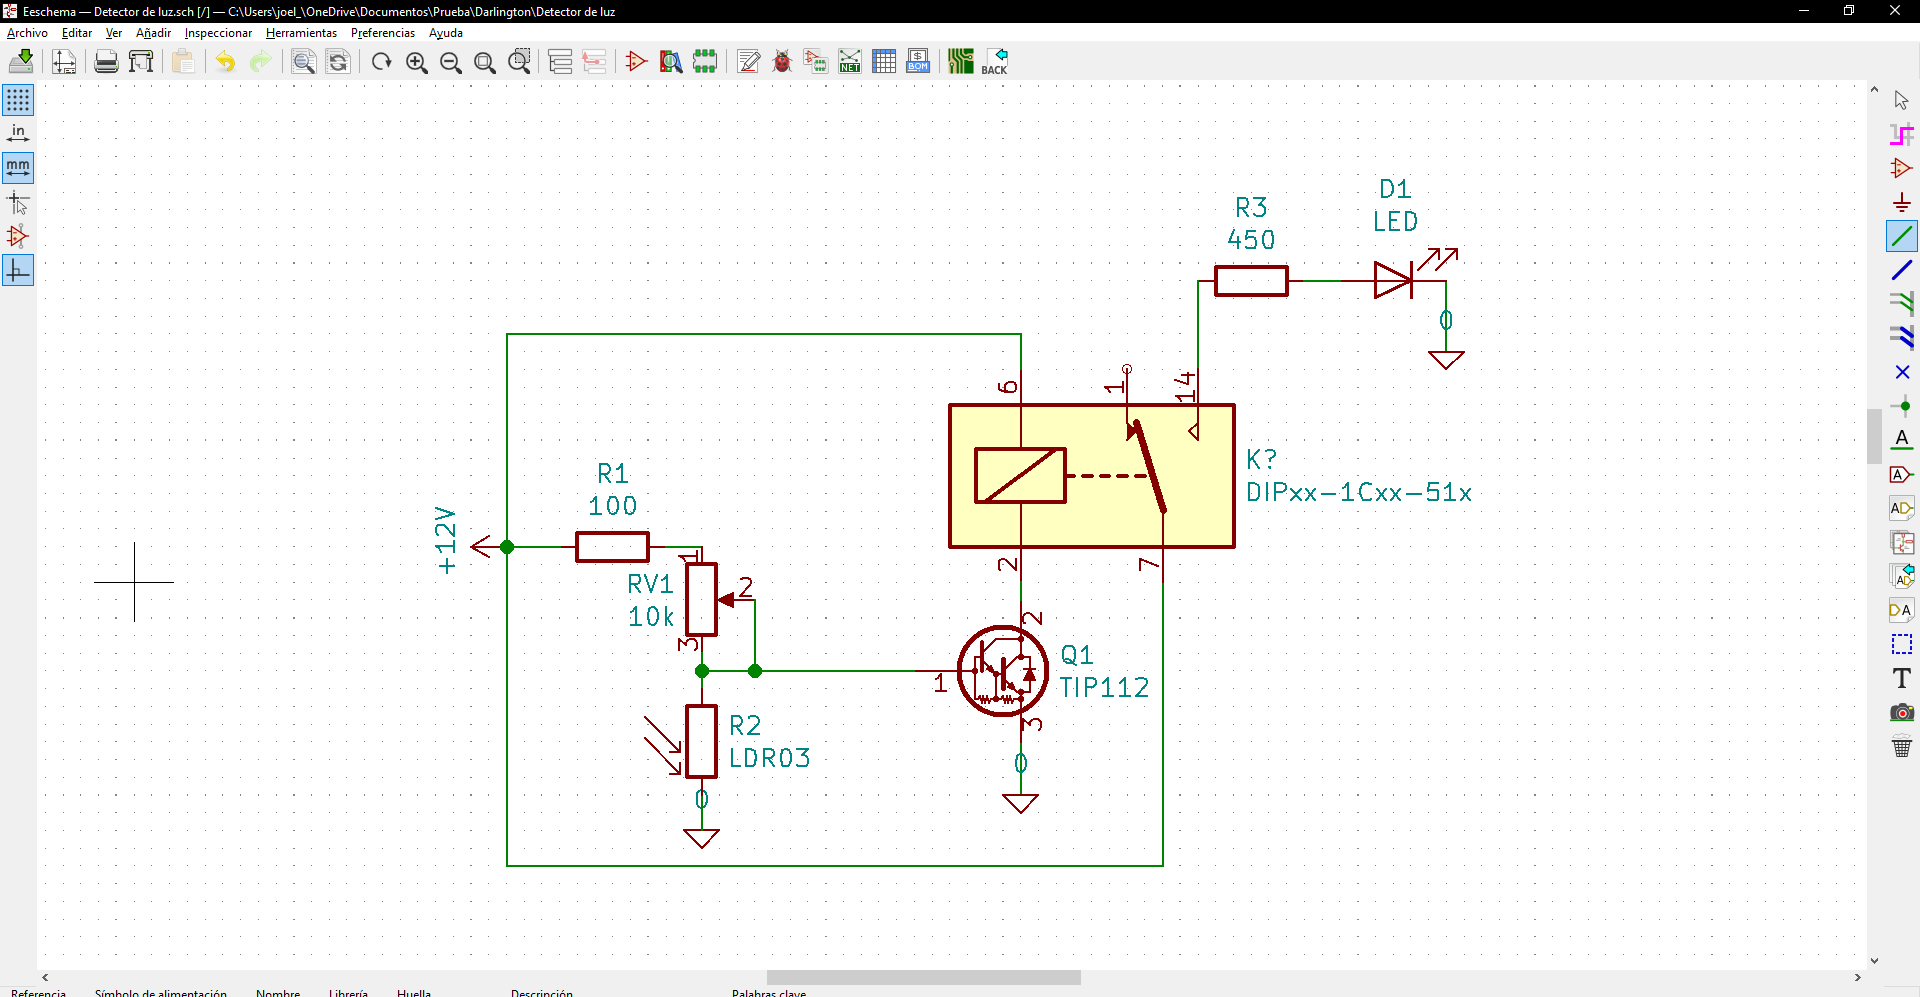
\includegraphics[scale=0.2]{IMG/circomp.png}
            \caption{Circuito completo}
            \label{fig:my_label}
        \end{figure}
        \item Se ajusta el potenciómetro para la cantidad de luz deseada.
    \end{enumerate}
\end{large}
\section{Procedimiento: Circuito de activación.}
\begin{large}
    \begin{enumerate}
        \item Se calcula la resistencia del arduino al darlington con la formula vista previamente, entonces:\\\\
        $\frac{(5-0.7)1000}{0.4}=10750\Omega$\\\\
        \item se coloca la resistencia del valor mas cercano al resultado en la base siguiendo el esquema de la figura 4.
        \begin{figure}[htbp]
            \centering
            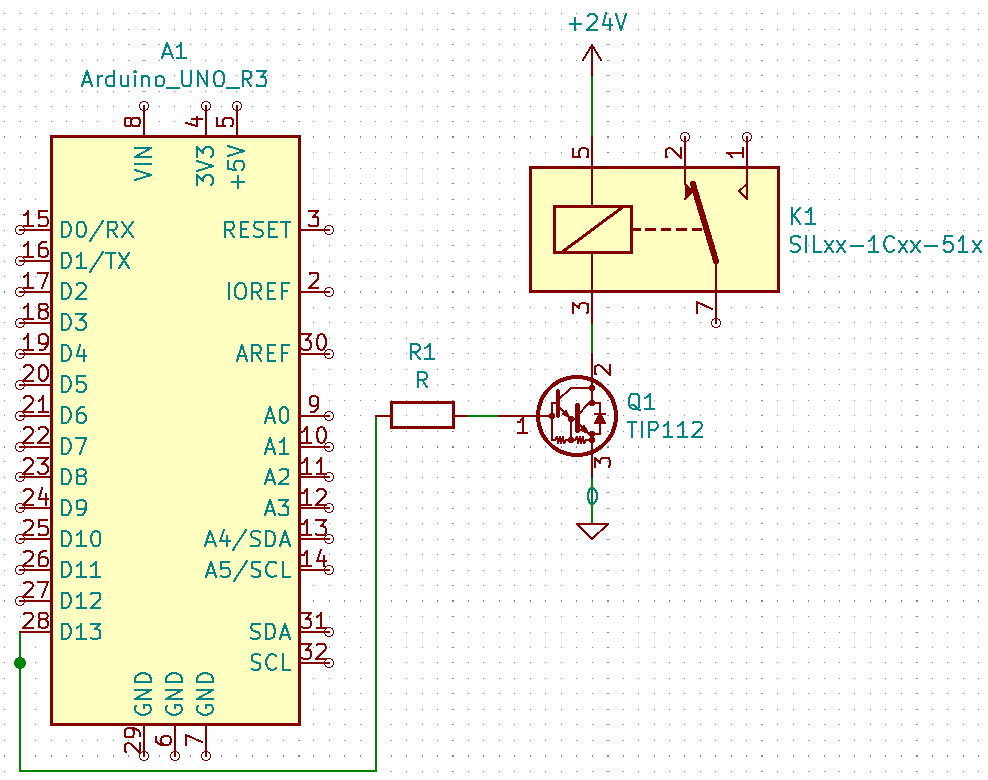
\includegraphics[scale=0.4]{IMG/ciract.png}
            \caption{Circuito de activación.}
        \end{figure}
    \end{enumerate}
\end{large}
\section{Resultados:}
Cómo resultados el movimiento del relay de normalmente cerrado a normalmante abierto es efectuado; esto gracias al trabajo del darlingron para amplificar la salida y a su vez permitir el paso de la corriente. 
Como se puede ver en la siguiente figura:\\
\begin{figure}[htbp]
    \centering
    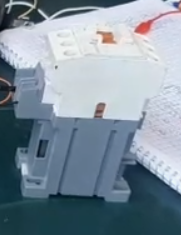
\includegraphics[width=5cm]{IMG/releisoteOn.PNG}
    \caption{Abierto}
    \label{fig:On}
\end{figure}

\begin{figure}[htbp]
    \centering
    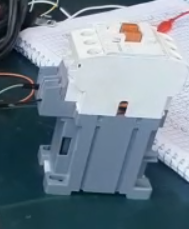
\includegraphics[width=5cm]{IMG/releisoteOff.PNG}\\
    \caption{Cerrado}
    \label{fig:OFF}
\end{figure}
\newpage
\begin{large}
    De igual manera en el circuito detector de luz se logra activar la bobina del relay dependiendo de la luz recibida por el LDR, esto como consecuencia de el circuito divisor de corriente como se muestra en la figura 7.\\
    \begin{figure}[htbp]
        \centering
        \subfigure[Circuito con sombra]{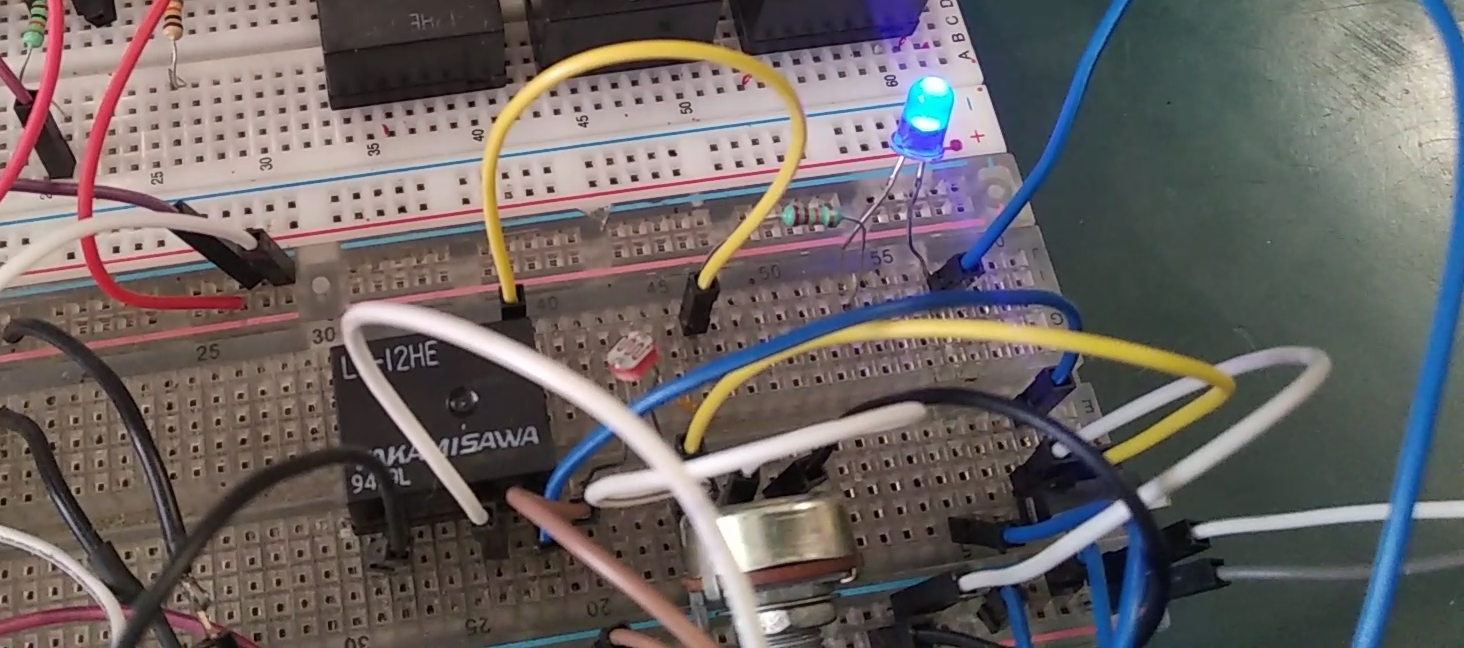
\includegraphics[width=8cm]{IMG/rt4.png}}
        \subfigure[Circuito sin sombra]{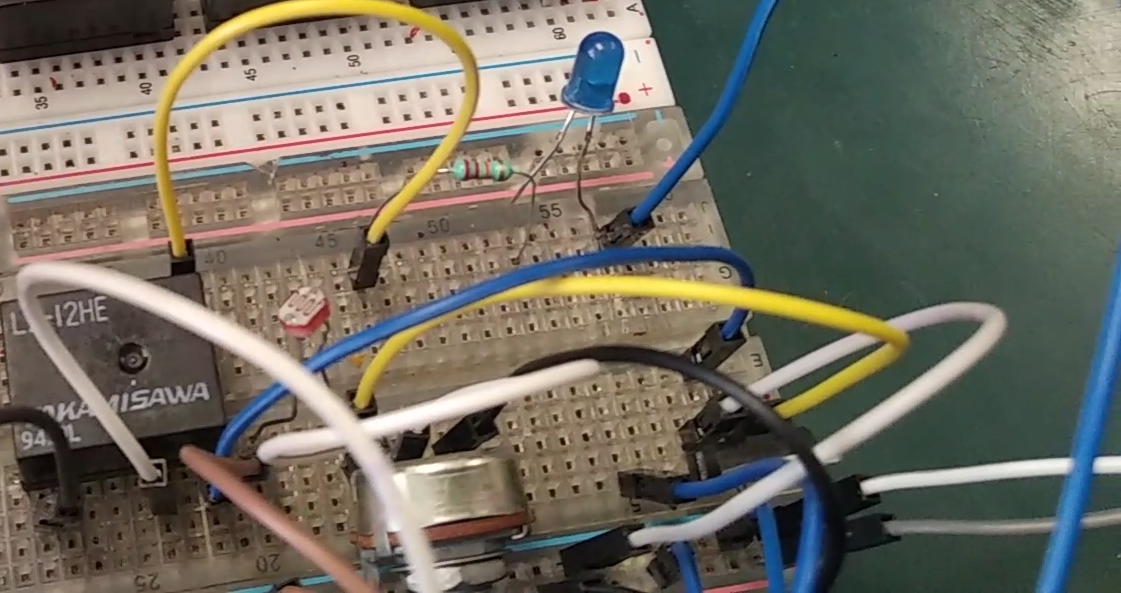
\includegraphics[width=8cm]{IMG/rt3.png}}
        \caption{Estados del circuito ante la luz.}
    \end{figure}
\end{large}
\section{Conclusiones:}
En conclusión se aprendió sobre el uso del Darlington cómo switch y como amplificador, así como su arquitectura y los posibles "remplazos" que podría tener, así en caso de no tener un Tip112 poder crear un amplificador con el uso de dos TIP41C.\\
Los usos de los transistores son muy variados y entre ellos se encuentra su funcion de switch que es muy util por su tiempo de reaccion y las velocidades que pueden alcanzar al ser dopados que aunque no es la misma que un mosfet si es muy alta, la ventaja de un transistir darlington es que puede amplificar mucho mas que un transistor normal al ser 2 transistores unidos basicamente, esto perimite que las seales que entran a el sean muy bajas sin problema.

\end{document}
